% Tamanhos
% \tiny
% \scriptsize
% \footnotesize
% \small 
% \normalsize
% \large 
% \Large 
% \LARGE 
% \huge
% \Huge

% Posicionamento
% \centering 
% \raggedright
% \raggedleft
% \vfill 
% \hfill 
% \vspace{Xcm}   % Colocar * caso esteja no começo de uma página. Ex: \vspace*{...}
% \hspace{Xcm}

% Estilo de página
% \thispagestyle{<<nosso>>}
% \thispagestyle{empty}
% \thispagestyle{plain}  (só número, sem cabeço)
% https://www.overleaf.com/learn/latex/Headers_and_footers

% Compilador que permite usar fonte de sistema: xelatex, lualatex
% Compilador que não permite usar fonte de sistema: latex, pdflatex

% Definindo fontes
% \setmainfont{Times New Roman}  % Todo o texto
% \newfontfamily\avenir{Avenir}  % Contexto

\begingroup\thispagestyle{empty}\vspace*{.05\textheight} 

              % \formular
              % \LARGE 
              % \begin{center}
              % \textsc{Ação direta e\\outros escritos}
              % \end{center}
              % \smallskip

\section {Mesa de jantar Luís XV com seis cadeiras}

\begin{figure}[htpb!]
\thisfloatpagestyle{empty}
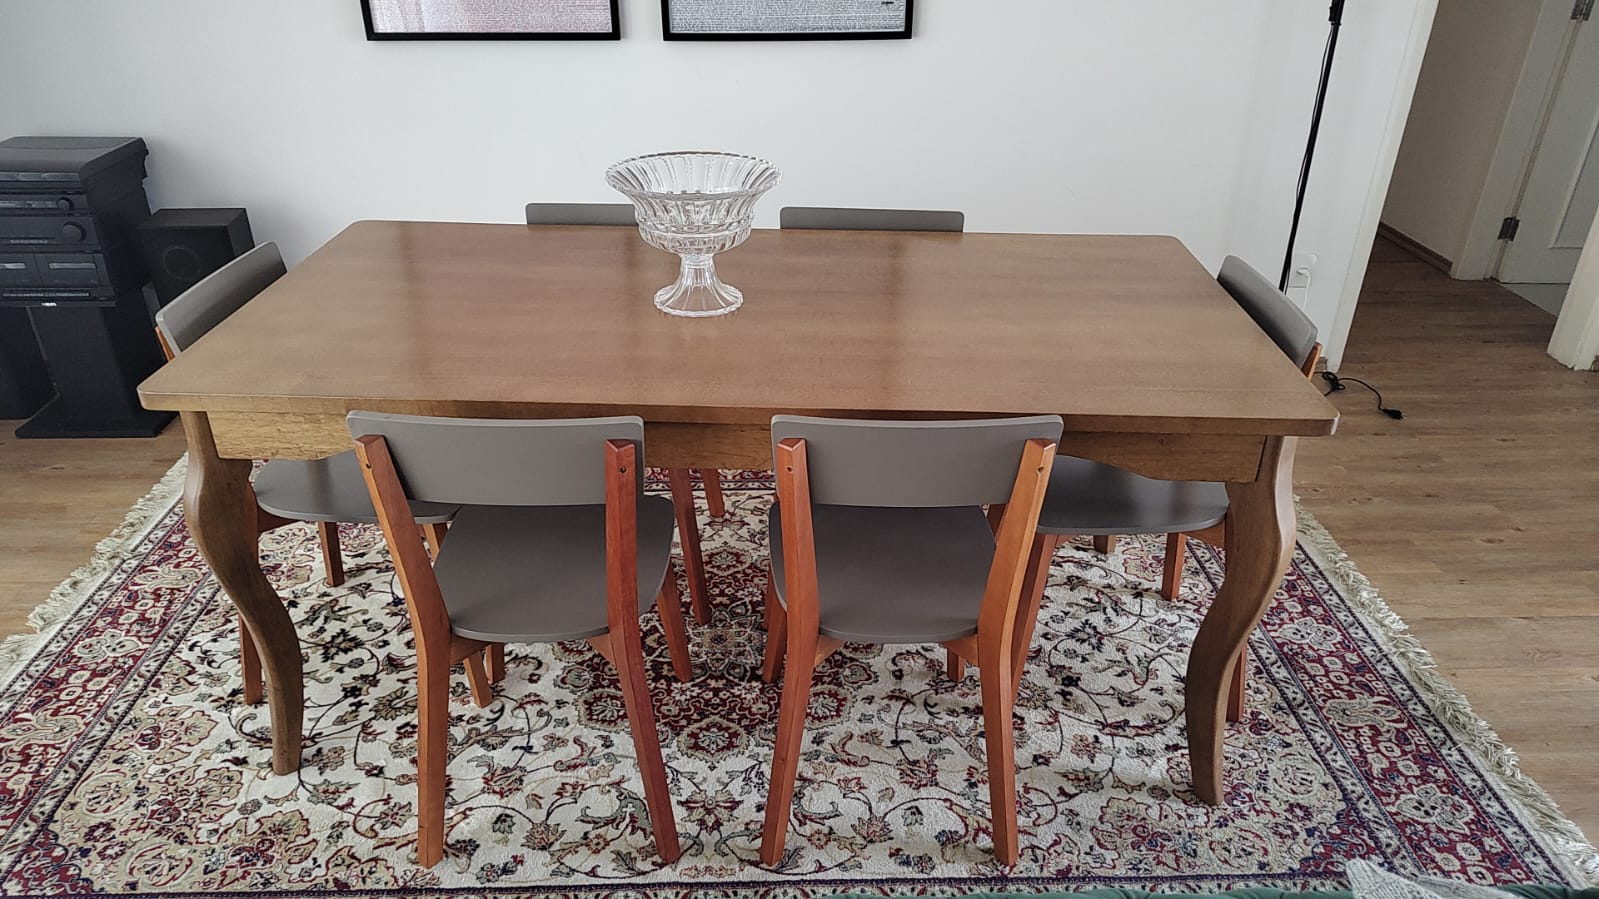
\includegraphics[width=\textwidth]{./MEDIA/MESA_JANTAR.jpeg}
\caption{Mesa de jantar Luís XV com seis cadeiras.}
\end{figure}

\textbf{Medidas}
\begin{itemize}
\item Largura: 180 cm (em torno de)
\item Altura: 100 cm (em torno de)
\end{itemize}

\textbf{Valor}
\begin{itemize}
\item 1.900 reais
\end{itemize}
                    
\endgroup
\vfill
\pagebreak